\documentclass[12pt]{article}

\usepackage[utf8]{inputenc}
\usepackage[russian]{babel}

\usepackage{amssymb}
\usepackage{amsmath}
\usepackage{amscd}
\usepackage{amsthm}
\usepackage{xcolor}

\usepackage{indentfirst}

%\usepackage{marginnote} % this is used for notes on the right margin --- \marginnote{\footnotesize txt}

\usepackage{mathtools} % for mathclap command

%\usepackage[normalem]{ulem} % for crossing text out - \sout

% Redefining \def is impossible. I tried, but it is impossible.
%\let\def_prev\def

%%%%%%%%%%%%%%%%%%%%%%%%%%%%%%%%%%%%%%%%%%%%%%%
%           MATH OPERATORS SPACING            %
%%%%%%%%%%%%%%%%%%%%%%%%%%%%%%%%%%%%%%%%%%%%%%%

\let\existstemp\exists
\let\foralltemp\forall
\renewcommand{\exists}{\: \existstemp \:}
\newcommand{\existsonly}{\: \existstemp ! \:}
\renewcommand{\forall}{\: \foralltemp \:}

%%%%%%%%%%%%%%%%%%%%%%%%%%%%%%%%%%%%%%%%%%%%%%%
%            COMMAND SHORTHANDS               %
%%%%%%%%%%%%%%%%%%%%%%%%%%%%%%%%%%%%%%%%%%%%%%%

\newcommand{\example}{{\itshape Пример. }}
\newcommand{\equals}{\Leftrightarrow}
\newcommand{\exc}{{\bfseries Упражнение. }}
\newcommand{\norm}[1]{\left\| #1 \right\|}
\newcommand{\scal}[2]{\left\langle #1, #2 \right\rangle}
\newcommand{\angular}[1]{\langle #1 \rangle}

\newcommand{\Sum}[2]{\underset{#1}{\overset{#2}{\sum}}}
\newcommand{\Int}[2]{\underset{#1}{\overset{#2}{\int}}}
\newcommand{\Ker}{\text{Ker}}

% Physicists' variant of dot product
\newcommand{\pscal}[2]{\, \langle #1 | #2 \rangle \,}
\newcommand{\bra}[1]{\, \langle #1 |}
\newcommand{\ket}[1]{| #1 \rangle \,}

\renewcommand{\leq}{\leqslant}
\renewcommand{\geq}{\geqslant}

%%%%%%%%%%%%%%%%%%%%%%%%%%%%%%%%%%%%%%%%%%%%%%%
%         THEOREM DEFINITION LINES            %
%%%%%%%%%%%%%%%%%%%%%%%%%%%%%%%%%%%%%%%%%%%%%%%

\newtheorem{lem}{Лемма}[section]
\newtheorem{note}{Замечание}[section]
\newtheorem{defi}{Определение}[section]
\newtheorem{theorem}{Теорема}[section]
\newtheorem{state}{Утверждение}[section] % statement

%%%%%%%%%%%%%%%%%%%%%%%%%%%%%%%%%%%%%%%%%%%%%%%
%             GRAPHICS INCLUSION              %
%%%%%%%%%%%%%%%%%%%%%%%%%%%%%%%%%%%%%%%%%%%%%%%

\usepackage{graphicx}

\graphicspath{{./Graphics/}}

%%%%%%%%%%%%%%%%%%%%%%%%%%%%%%%%%%%%%%%%%%%%%%%
%               DRAFT TEMPLATES               %
%%%%%%%%%%%%%%%%%%%%%%%%%%%%%%%%%%%%%%%%%%%%%%%

%\usepackage{marginnotes}
\newcommand{\todo}[1]{\marginpar{\color{red} \tiny #1}}

\begin{document}

\section{Операторы в гильбертовых пространствах}

	% Излишняя информация: и так очевидно, что многие обозначения не унифицированы.
	%Прежде чем начать изучение линейных операторов, стоит предупредить, что буквы, используемые нами для обозначения некоторых
	%классических операторов, могут не являться общепринятыми и отличаться от принятых в различной литературе по данному предмету.
	
	\begin{defi}
		Отображение $A$ из $M$ в $L$ назовём \textbf{линейным оператором}, если область определения оператора
		$D(A) \subset M$ и выполнены следующие условия:
		\begin{enumerate}
			\item $A(x + y) = Ax + Ay$
			\item $A(\alpha x) = \alpha A x$ 
		\end{enumerate}
		Обозначают $A : M \rightarrow L$.
	\end{defi}
	
	Впрочем, определение линейного оператора уже рассматривалось в курсе линейной алгебры. При рассмотрении линейных операторов в
	нашем курсе, будем предполагать, что $M$ и $L$ --- нормированные пространства. А если есть норма $\Rightarrow$ есть расстояние
	$\Rightarrow$ может быть определена непрерывность. Если $A$ непрерывно в $h_0$, пишут:
	
	$$ \forall \varepsilon > 0 \exists \delta > 0 : \forall h \: \norm{h - h_0} < \delta \Rightarrow \norm{Ah - Ah_0} 
	= \norm{A(h-h_0)} < \varepsilon $$
	Нетрудно видеть, что из непрерывности в точке следует непрерывность в нуле --- для этого нужно взять $h := h + h_0$. 
	Так же можно сделать для любой точки множества. Значит, $A$ непрерывна на всём множестве. Тогда, исходя из данного
	определения, получаем равномерную непрерывность для $A$.
	
	Приведём некоторые примеры линейных операторов:
	\begin{itemize}
		\item Тождественный оператор
		\item Нулевой оператор
		\item Оператор проектирования на замкнутое подпространство гильбертова пространства.
		\item $f(t) \rightarrow t \cdot f(t)$ в пространстве $\mathbb{L}_2 (0,1) \rightarrow \mathbb{L}_2 (0,1)$
		\item Оператор дифференцирования: $\mathsf{D}: \mathbb{L}_2 (0,1) \rightarrow \mathbb{L}_2 (0,1)$. Отметим также, что
		область определения этого оператора $D(\mathsf{D}) \neq \mathbb{L}_2 (0,1)$
		\item $f(x) \rightarrow \int_0^x f(t) dt$.
	\end{itemize}
	
	Для существования обратного оператора $A^{-1}$ нужно:
	\begin{enumerate}
		\item $A$ - инъективно.
		\item $D(A^{-1}) = $ образ прямого отображения
	\end{enumerate}
	В наших обозначениях, обратный оператор всегда определяет обратное отображение. 
	\off{В некоторых книгах это может быть не так.}

	\subsection{Ограниченный линейный оператор}	
	
		% Является менее удачным вариантом следующего определения
		%\begin{defi}
		%	Множество ограничено, если существет шар с центром в точке $O$, в котором содержится все множество.
		%\end{defi}
		\begin{defi}
			Множество $M$ \textbf{ограничено}, если существует шар $B_r(a)$, в котором содержится все множество:
			$$ \exists a \in X \; \exists (r > 0) \; \forall x \in X (x \in M \Rightarrow \rho(a, x) < r) $$
		\end{defi}
		\begin{defi}
			Оператор $A: M \Rightarrow L$ называется \textbf{ограниченным}, если он переводит любое ограниченное множество
			в ограниченное.
		\end{defi}
	
		\begin{state}
			Линейный оператор ограничен $\equals$ он непрерывен.
		\end{state}
		\begin{proof}
			\textbf{Необходимость}. Если $A$ --- непрерывный оператор, то 
			$ \exists \delta : \norm{h} < \delta \Rightarrow \norm{Ah} < 1 $. (Для удобства в определении 
			непрерывного оператора взяли $\varepsilon = 1$.)
			
			Возьмём ограниченное множество $\norm{h} < R$.
		
			Рассмотрим вектор $x = \frac{\delta h}{R}$. В указанных условиях
			$\norm{x} < R$, откуда следует $\norm{Ax} < 1$ и, из линейности оператора и свойств нормы:

			$$\frac{\delta}{R} \cdot \norm {Ah} < 1$$

			Это означает, что отображение $A$ переводит все значения в шар радиуса $\frac{R}{\delta}$, значит
			$A$ --- ограниченный оператор. \\
		
			\textbf{Достаточность}. Аналогично доказательству необходимости. Если $A$ --- ограниченный оператор,
			то при $\norm{h} \leq 1$ получается $\norm{Ah} \leq R$. Возьмём шар радиуса $\frac{\varepsilon}{R}$
			и действуем так же, как в предыдущем доказательстве.
		\end{proof}
	
	\subsection{Норма линейного оператора}
	
		\begin{defi}
			\textbf{Нормой линейного оператора} $A$ называется следующая величина: 
			$$\norm{A} \overset{df}{=} \underset{x \neq 0}{sup} \frac{\norm{Ax}}{\norm{x}}$$
		\end{defi}
	
		\begin{state}
			Линейный оператор ограничен $\equals$ его норма конечна.
		\end{state}
		\begin{proof}
			Распишем норму линейного оператора:
			$$
				\norm{A} \overset{df}{=} \underset{x \neq 0}{sup} \frac{\norm{Ax}}{\norm{x}} = 
				\underset{x \neq 0}{sup} \norm{A \frac{x}{\norm{x}}} =
				\underset{\norm{y} = 1}{sup} \norm{Ay} \leq
			$$
			$$
				\leq
				\underset{0 < \norm{y} \leq 1}{sup} \norm{Ay} \leq
				\underset{0 < \norm{y} \leq 1}{sup} \frac{\norm{Ay}}{\norm{y}} \leq
				\underset{y \neq 0}{sup} \frac{\norm{Ay}}{\norm{y}} =
				\norm{A}
			$$
			Так как все неравенства, приведенные здесь, были направлены в одну сторону,
			они обратятся в равенства. При этом, последнее равенство гарантирует, что
			оператор $A$ переведёт вектор $\norm{h} \leq r$ в замкнутый шар радиуса $\norm{A} \cdot r$.
			С другой стороны, при ограниченности оператора, его норма будет конечна, по приведённым
			выше равенствам.
		\end{proof}
	
		Сделаем также ещё одно замечание, исходящее из определения:
		$$ \frac{\norm{Ax}}{\norm{x}} \leq \norm{A} $$
		$$ \norm{Ax} \leq \norm{A} \cdot \norm{x} $$
	
		Мы в очередной раз что-то назвали нормой. Но {\color{gray}гуманно} верно ли это?
	
		\exc Для нормы линейного оператора выполнены все аксиомы нормы.
		% TODO: потом хотелось бы написать здесь доказательство и переписать это как "Утверждение".
	
		Также остается упражнение по доказательству еще одного полезного свойства:

		\exc Доказать выполнение равенства $\norm{A} - \norm{B} \leq \norm{A-B}$.
	
		\begin{state}
			$$\norm{Ax} \leq k \norm{x} \Rightarrow \norm{A} \leq k$$
		\end{state}
	
		\begin{state}
			Для нормы композиции линейных операторов верно неравенство 
			$$\norm{A\cdot B} \leq \norm{A} \cdot \norm{B}$$
		\end{state}
		\begin{proof}
			$$ \norm{(AB)x} = \norm{A(Bx)} \leq \norm{A} \cdot \norm{Bx} \leq \norm{x} \cdot \norm{A} \cdot \norm{B} $$
			Отсюда 
			$$ \norm{AB} \leq \norm{A} \cdot \norm{B},$$
			что и требовалось доказать. \\
		\end{proof}
	
	\subsection{Оператор Гильберта-Шмидта}
		Рассмотрим пространства $\mathbb{L}_2(\mathbb{R}^n)$ и $\mathbb{L}_2(\mathbb{R}^k)$, а также функцию
		$$ k(x,y) \in \mathbb{L}_2(\mathbb{R}^{n+k}), x \in \mathbb{R}^n, y \in \mathbb{R}^k$$
	
		\begin{defi}
			\textbf{Оператором Гильберта-Шмидта} назовём оператор:
			$$ (Af)(t) \overset{df}{=} \underset{\mathbb{R}^k}{\int} k(t,y) f(y) dy $$
		\end{defi}
	
		Покажем, что функция $(Af)(t)$ определена почти для всех $t$. Пользуясь определением скалярного произведения в $\mathbb{L}_2$, 
		видим, что $\mod{(Af)(t)}^2 = (\scal{f}{k})^2 \leq \norm{f}^2 \cdot \underset{\text{на }\mathbb{R}^k}{\norm{k}^2}$
	
		$$ \mod{(Af)(t)}^2 \leq \underset{\mathbb{R}^k}{\int} |f(y)|^2 dy \cdot \underset{\mathbb{R}^k}{\int} |k(t,y)|^2 dy $$
	
		Проинтегрируем обе части выражения по множеству $\mathbb{R}^n$:
	
		$$ \Int{\mathbb{R}^n}{} \mod{(Af)(t)}^2 \, dt \leq \underset{\mathbb{R}^k}{\int} |f(y)|^2 \, dy 
		   \cdot \Int{\mathbb{R}^n}{} \Int{\mathbb{R}^k}{} |k(t,y)|^2 \, dt \, dy $$
	
		$k(t,y)$ почти всюду определена в $\mathbb{R}^k$, интегрируема
		в $\mathbb{R}^k$ по условию. Значит, по теореме Фубини можем переставить пределы интегрирования 
		и перейти к норме на $\mathbb{R}^n$.
	
		$$ \Int{\mathbb{R}^n}{} \mod{(Af)(t)}^2 \, dt \leq \norm{f}^2_{\mathbb{L}_2} \cdot \norm{k}^2_{\mathbb{L}_2} $$

		\lecture{6}

		Как известно, в конечномерном пространстве все нормы являются эквивалентными. Но это отнюдь не является верным для бесконечномерных
		пространств.
	
		\todo{Переместить в ограниченность?}
		\example \textit{(Неограниченного оператора)}. Оператор дифференцирования 
		$\frac{d}{dx} : \mathbb{L}_2(0, 1) \rightarrow \mathbb{L}_2(0, 1)$ является неограниченным. 
		Достаточно рассмотреть $\norm{sin(nx)}_{\mathbb{L}_2} \leq 1$. При воздействии на синус оператором дифференцирования, получим
		$$|n \cdot cos(nx)| \geq n \cdot cos^2(nx) = n^2 \cdot \frac{1 + cos(2nx)}{2}$$
		Таким образом, легко увидеть неограниченность нормы $n \cdot cos(nx)$:
		\begin{align*}
			\norm{n \cdot cos(nx)}_{\mathbb{L}_2(0,1)}^2 
			&\geq \frac{n^2}{4} \Int{0}{1} \big(1 + 2 cos(2nx) + cos^2(2nx)\big) dx \geq \\
			&\geq \frac{n^2}{4} \Int{0}{1} \big(1 + 2 cos(2nx)\big) dx \geq \frac{n^2}{4} - 1
		\end{align*}
		При $n \rightarrow \infty$ этот образ не попадает в конечный шар, значит оператор $\frac{d}{dx}$ неограничен.
	
		% Доразобраться
	
	\subsection{Продолжение линейного оператора}

		\todo{Уточнить формулировку.}
		\off{Скорее всего, здесь утверждается, что $\existsonly A_2$. Надо уточнить.}
		\begin{theorem} \label{th:limitedOperContinue}
			Рассмотрим линейный оператор $A_1 : E \rightarrow F$. Если выполнены следующие условия:
			\begin{enumerate}
				\item $F$ --- полное.
				\item $D(A_1) = E_1 \subset E_2$.
				\item $\overline{E}_1 \supset E_2$ (То есть $E_1$ плотно в $E_2$).
			\end{enumerate}
			То найдётся линейный оператор $A_2,\, D(A_2) = E_2$, такой, что: \\
			$\norm{A_2} \leq \norm{A_1}$ \\
			$A_2 \lims{E_1}{} = A_1$
		\end{theorem}
	
		\begin{proof}
			%   УБРАНО, ТАК КАК ИЗЛИШНЕ МНОГОСЛОВНО   %
			%Введём $x \in E_2, x_i \in E_1$. Пусть элементы $x_i$ образуют фундаментальную последовательность. Так как $E_1$ плотно в $E_2$,
			%то найдётся элемент $x \in E_2$, являющийся пределом последовательности $x_1, ..., x_n, ...$.
			Докажем по пунктам:
			\begin{itemize}
				\item $A_2 \lims{E_1}{} = A_1$ \\
				Положим $x_i \in E_1$, $\{x_n\}$ --- фундаментальная последовательность. Так как $E_1$ плотно в $E_2$, то
				$\lim x_n = x\in E_2$. Воздействуем на нашу последовательность оператором $A_1$.
				Последовательность $\{A_1 x_n\}$ останется фундаментальной. Так как $F$ --- полное пространство, 
				то любая фундаментальная последовательность в нём будет иметь предел:
		
				$$A_1x_n \rightarrow y \qquad y \in F$$
				Тогда, для любых $x \in E_2 \textbackslash E_1$, можно определить $A_2 x = y$. Осталось только 
				показать, что для предельных точек $A_2$ будет линейным оператором.
		
				Достаточно взять $z = \alpha x + \beta y$ и сходящуюся к нему последовательность $z_n = \alpha x_n + \beta y_n$.
				Воздействуя оператором $A_1$ на $z_n$, получаем выражение:
				$$A_1 z_n = \alpha A_1 x_n + \beta A_1 y_n$$
				В пределе, при $n \rightarrow \infty$, равенство преобразуется следующим образом:
				$$A_2 z = \alpha A_2 x + \beta A_2 y$$
			
				\off{По всей видимости, показали, что $A_2$ определяется однозначно и является линейным.}
			
				\item $\norm{A_2} \leq \norm{A_1}$ \\
				Другими словами, ограниченность оператора $A_1$ влечёт ограниченность оператора $A_2$. Рассмотрим следующее 
				неравенство:
				$$\norm{A_1 x_n} \leq \norm{A_1} \cdot \norm{x_n}$$
				В пределе $A_1 x_n \underset{n \rightarrow \infty}{\rightarrow} A_2 x$. Тогда
		
				$$\norm{A_2 x} \leq \norm{A_1} \cdot \norm{x}$$
		
				То есть $\norm{A_2} \leq \norm{A_1}$. С другой стороны 
				$\norm{A_2} = \underset{x\neq 0}{\sup} \frac{\norm{A_2x}}{\norm{x}} \geq \norm{A_1}$
				Таким образом, $\norm{A_1} = \norm{A_2}$.
			\end{itemize}
		\end{proof}
	
	\subsection{Предел и сходимость}

		Введём определение предела последовательности оператора. Стоит отметить, что в различной литературе данное определение может вводиться
		по-разному.
	
		\begin{defi}
			$A$ является \textbf{пределом} $A_n$, если $D(A_n)=E' \in E$ (определены на одном и том же подмножестве $E$) и:
		
			$$\forall x \in E, A_n x \underset{n \rightarrow \infty}{\rightarrow} A x$$
		\end{defi}
		В нормированных пространствах вводится еще один 
		важный термин:
	
		\begin{defi}
			Если для линейного оператора $A$ и последовательности линейных операторов $A_n$ имеет место:
			$$\norm{A_n - A} \rightarrow 0$$
			то $A_n$ \textbf{равномерно сходится} к $A$, что обозначается как $A_n \rightrightarrows A$.
		\end{defi}
	
		Легко показать, что равномерная сходимость всегда влечёт обычную. Действительно, рассмотрим
		$$\norm{A_n x - A x} \leq \norm{A_n - A} \cdot \norm{x} \rightarrow 0$$
		Отсюда следует $\forall x, A_n x \rightarrow A x$, что является определением сходимости линейных операторов.
		%\begin{state}
		%	Равномерная сходимость линейных операторов влечёт обычную.
		%\end{state}
	
		В приведённых выше рассуждениях есть одна неочевидная деталь --- предел последовательности элементов не обязательно должен лежать
		в том же множестве, что и элементы последовательности. Является ли $A$, как предел $A_n$ линейным оператором?
	
		\begin{state}
			Предел последовательности линейных операторов является линейным оператором.
		\end{state}
		\begin{proof}
			Проверим, обладает ли $A$ свойствами линейного оператора. Рассмотрим вектор $z = \alpha x + \beta y$. 
			Тогда, пользуясь линейностью операторов из последовательности $A_n$:
			$$ A_n \cdot z \rightarrow A \cdot z $$
			$$ \alpha A_n x + \beta A_n y \rightarrow \alpha A x + \beta A y $$
			Значит, верно равенство $A(\alpha x + \beta y) = \alpha A x + \beta A y$ и $A$ является линейным оператором.
		\end{proof}
	
		Определить ограниченность оператора $A$, исходя из свойств последовательности $A_n$ намного сложнее, но легко 
		установим следующий факт:
		\begin{state}
			Если $A_n \rightarrow A$ и $\forall n \norm{A_n} \leq C$, где $C$ --- некоторая константа, то 
			оператор $A$ является ограниченным.
		\end{state} 
		\begin{proof}
			\todo{Миша, тебе нельзя лениться. Ты же умничка!}
			Очевидно. {\color{gray}Sorry, но я и так умаялся предыдущее доказательство писать, а оно тоже очевидное.}
		\end{proof}

		\example $P_n : l_2 \rightarrow l_2$ --- оператор проектирования на n-мерное подпространство.
		$$P_n : (x_1, \dots , x_n, x_{n+1}, \dots) \longmapsto (x_1, \dots, x_n, 0, 0, 0, \dots)$$
		Рассматривая свойства пространства $l_2$, легко понять, что $P_n \rightarrow I$. Действительно, так как $x_n$ --- элементы 
		сходящегося ряда, то норма <<хвоста>> этого ряда будет стремиться к нулю.
		%\marginnote{\footnotesize I --- тождественный оператор}[-1.5cm]
		Но, в то же время, равномерной сходимости не достигается: $\norm{P_n - I} = 1$. Следовательно, обычная сходимость не влечёт
		равномерную.
	
		\exc Пусть $A_n \rightrightarrows A, B_n \rightrightarrows B$. Доказать $A_n B_n \rightrightarrows A B$. 
		(Разумеется, доказывается данное утверждение в предположении, что композиция $A B$ существует, то есть совпадают область определения
		A и множество значений B.)
	
		\begin{state}
			Рассмотрим последовательность $A_n : E \rightarrow F$. Утверждается, что, если $F$ --- полное, то пространство 
			ограниченных линейных операторов $\{A_n\}$ образует полное нормированное пространство.
		\end{state}
		\begin{proof}
			Возьмём $A_n$ --- фундаментальную последовательность, тогда $\norm{A_n - A_m} \rightarrow 0$, отсюда следует, что 
			$A_n \cdot x$ --- фундаментальная последовательность и, так как $F$ --- полное множество, она имеет предел, который
			мы обозначим за $A \cdot x$ ($\forall x \: A_n \cdot x \rightarrow A \cdot x$).
		
			\textbf{Линейность.} Ранее уже было доказано, что предел последовательности линейных операторов также является линейным
			оператором.
		
			\textbf{Ограниченность.} Так как последовательность является фундаментальной, можем ограничить норму разности её элементов 
			с достаточно большими номерами константой.
			$$\forall n,m > N,\,\,\norm{A_n - A_m} \leq 1$$
			Тогда, применяя неравенство треугольника, легко приходим к доказательству ограниченности оператора:
			$$\norm{A_n} \leq 1 + \norm{A_m}$$
		
			\textbf{Равномерная сходимость.} По определению фундаментальной последовательности:
			$$
				\norm{A_n - A_m} \rightarrow 0 \overset{df}{\equals} 
				\forall \varepsilon > 0\, \exists N_0\, \forall m, n \geq N_0 \; \norm{A_n - A_m} < \varepsilon
			$$
			В силу $A_n \rightrightarrows A$, получаем, в таких же обозначениях:
			$$ \norm{A_n - A} \leq \varepsilon $$
			Данное неравенство при $\varepsilon \rightarrow 0$ является определением равномерной сходимости.
		
			Таким образом, $\{A_n\}$ обладает всеми свойствами, нужными для того, чтобы пространство являлось полным, что и требовалось 
			доказать.
		\end{proof}
	
		\begin{defi}
			Если для полного пространства $F$ и операторов $A_n : E \rightarrow F$ имеет место предельное соотношение
			$$\Sum{n=1}{N} A_n \underset{N \rightarrow \infty}{\rightarrow} A,$$
			то оператор $A = \Sum{n=1}{\infty} A_n$ называют \textbf{операторным рядом}.
		\end{defi}
	
		Определим для подобного ряда критерий Коши (критерий сходимости фундаментальной последовательности):
		$$\forall \varepsilon > 0 \; \exists N(\varepsilon) \; m > n > N(\varepsilon) \; \norm{ \Sum{n}{m} A_i } < \varepsilon$$
	
		Операторный ряд является одним из способов построения функции от операторов. Но данным способом могут быть выражены только 
		аналитические функции.
	
		\example Пусть $A$ --- ограниченный линейный оператор. Тогда ряд 
		$$\Sum{n = 0}{\infty} \frac{A^n}{n!}$$
		сходится, так как $\norm{A^n} \leq \norm{A}^n$, а ряд $\Sum{n=0}{\infty} \frac{\norm{A}^n}{n!}$ ничем не отличается от ряда
		$\Sum{n=0}{\infty} \frac{t^n}{n!}$, обладающего радиусом сходимости $R = \infty$.
	
	\subsection{Обратный оператор}
	
		Чтобы существовало обратное отображение $A^{-1}$, необходима инъективность оператора $A$. Более формально это записывается так: \\
		Пусть $A : E \rightarrow F$ и $A$ --- инъективен $\Rightarrow \exists A^{-1}, D(A^{-1}) = \Im(A)$.
	
		\begin{state}
			$A^{-1}$ аддитивен и однороден.
		\end{state}
		\begin{proof}
			\textbf{Аддитивность.} Рассмотрим вектора $y \in \Im(A),\, z~\in~\Im(A)$, тогда по линейности $A$, $y + z \in \Im(A)$.
			Определим вектор $x$:
			$$x = A^{-1}(y + z) - A^{-1} y - A^{-1} z$$
			Воздействуем на него оператором A, учитывая, что $A A^{-1} = I$.
			$$Ax = I(y + z) - I y - I z = 0$$
			Таким образом, из линейности оператора $A$, $x = 0$, что доказывает аддитивность обратного оператора.
		
			\textbf{Однородность.} Опять же, рассмотрим $y \in \Im(A)$ и определим вектор $x$:
			$$ x = A^{-1}(\lambda y) - \lambda A^{-1} y $$
			$$ Ax = \lambda y - \lambda y = 0 $$
			Следовательно, $x = 0$, поэтому $A^{-1}$ однородно.
		
			Доказаны аддитивность и однородность $\Rightarrow$ оператор $A^{-1}$ линеен.
		\end{proof}
	
		Ограниченность оператора $A$ отнюдь не влечёт ограниченность $A^{-1}$.
	
		\begin{theorem}
			(Без доказательства) Если $A$ --- линеен, ограничен и отображает полное нормированное пространство на полное нормированное
			пространство, то $\exists A^{-1}$ --- линейный и ограниченный оператор.
		\end{theorem}
	
		Пусть $A$ --- линейный оператор и $$\exists m > 0 : \forall x \; \norm {Ax} \geq m \cdot \norm{x}$$
		Это будет означать, что $A$ --- инъективный оператор, так как
		$$\norm{A(x-y)} \geq m \cdot \norm{x - y}$$
		Из этого неравенства следует, что, если $Ax = Ay$, то $x = y$. И, разумеется, инъективность оператора будет означать его
		обратимость.
	
		В таких условиях, оператор $A^{-1}$ будет ограниченным:
		$$ x = A^{-1} y $$
		$$ \norm{A^{-1} y} \leq \frac{1}{m} \norm{y} $$
		И это, в силу определения нормы оператора, означает $$\norm{A} \leq \frac{1}{m}$$
	
		\begin{theorem}
			Пусть $F$ --- полное пространство, $A : F \rightarrow F$ --- линейный оператор, $\norm{A} < 1$.
			Тогда оператор $I_F - A$ является обратимым, причём обратный оператор определяется как:
			$$
				(I_F - A)^{-1} = \Sum{0}{\infty} A^n
			$$
		\end{theorem}
		Стоит отметить, что ряд $\Sum{0}{\infty} A^n$ будет сходиться, так как $\norm{A} < 1$. Более того, скорость
		сходимости этого ряда не хуже, чем у суммы бесконечно убывающей геометрической прогрессии.
		\begin{proof}
			Умножим $(I_F - A)$ на частичную сумму ряда $\Sum{0}{N} A^n$:
			$$ \left(\Sum{0}{N} A^n \right) \cdot (I_F - A) = I_F - A^{N+1} \rightarrow I_F $$
			Взяв $N \rightarrow \infty$ превратим предел в равенство; умножим обе части уравнения на $(I_F - A)^{-1}$. Получаем
			$$ \Sum{0}{\infty} A^n = (I_F - A)^{-1} $$
			что совпадает с формулой, указанной в теореме.
		\end{proof}
	
		\begin{state}
			$A$ --- обратим, $\Delta$ --- ограниченный оператор, $\norm{\Delta} < \frac{1}{\norm{A^{-1}}}$, тогда оператор 
			$A + \Delta$ будет обратимым.
		\end{state}
		\begin{proof}
			\todo{Пояснять ли замену знака?}
			Вынесем $A$ за скобки:
			$$ A + \Delta = A \cdot \underbrace{(I + A^{-1} \cdot \Delta)}_
			   { \mathclap{\text{Обратимо по предыдущей теореме.}} } 
			$$
		\end{proof}
	
	\subsection{Спектр линейного оператора}
	
		Рассмотрим $A : F \rightarrow F$:%, $F$ --- плотное пространство.
		$$(A - \lambda \cdot I) = \lambda \cdot \left(\frac{A}{\lambda} - I\right)$$
		Как видно из ранее приведённых теорем, оператор $(A - \lambda \cdot I)$ будет обратимым 
		при достаточно больших значениях $\mod{\lambda}$.
	
		Запишем все группы $\lambda$, определяемые свойствами оператора $(A - \lambda \cdot I)$
	
		\begin{center}
			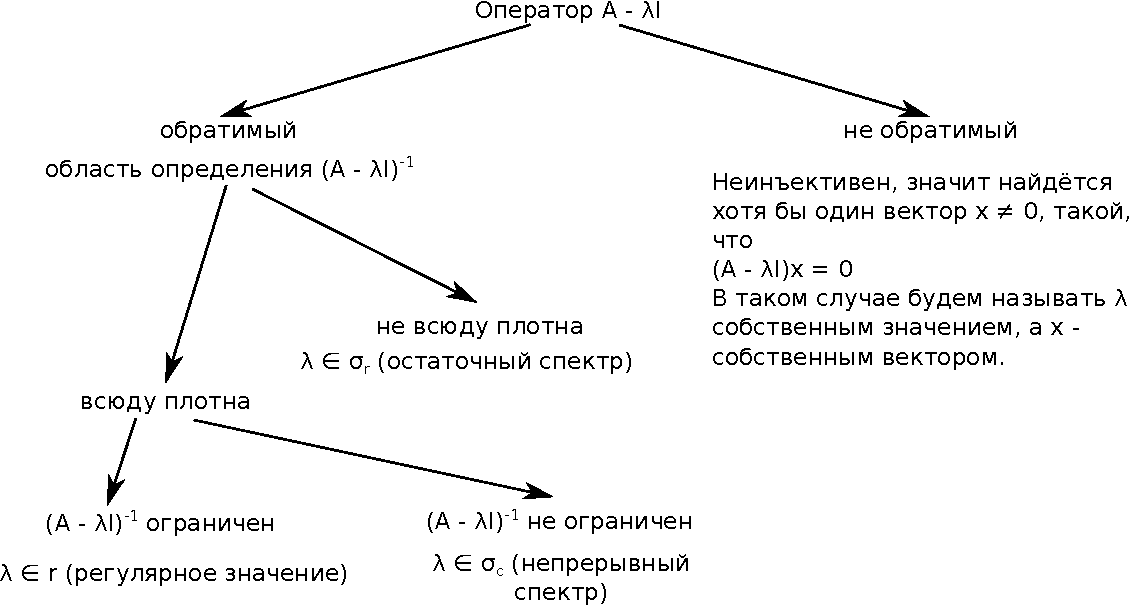
\includegraphics[width=1.0\linewidth]{../Graphics/Lectures-6-spectrum_scheme.pdf}\\
		\end{center}
	
		Для каждого $\lambda \in r(A)$ определяется ограниченный, с всюду плотной областью определения оператор
		$$ R_{\lambda} = (A - \lambda I)^{-1}$$
		Где $R_{\lambda}$ называется \textbf{резольвентным оператором} или \textbf{резольвентой}. \\
		Также отметим равенство, верное для любого линейного оператора:
		$$
			\overbrace{r(A)}^{ \mathclap{\text{Регулярные значения $A$}} } \cup 
			\underbrace{\sigma_1 (A) \cup \sigma_2 (A) \cup \sigma_3 (A)}_{\text{Спектр $A$}} = 
			r(A) \cup \sigma(A) = \mathbb{C}
		$$

		\lecture{7}

		% В конспекте упущено упоминание того, что было в прошлой лекции.

		%\subsection{Спектр и регулярные значения линейного оператора}
	
		На прошлой лекции был рассмотрен оператор $(A - \lambda I)$, и классификация значений $\lambda$, определяющаяся свойствами этого 
		оператора. Для удобства, в дальнейшем будем использовать обозначение $A_{\lambda} = (A - \lambda I)$.
	
		\begin{state}
			Множество регулярных значений $r(A)$ оператора $A$ является открытым.
		\end{state}
		\begin{proof}
			Ранее было доказано, что оператор $(A + \Delta)$ обратим, если $\norm{\Delta} \leq \frac{1}{\norm{A^{-1}}}$ 
			и $A$ является обратимым оператором. Тогда, если $\lambda \in r(A)$, то оператор
			$$ (A - \lambda I) - \mu I $$
			является обратимым для малых $\mu$. Этим доказывается открытость множества $r(A)$.
		\end{proof}
		С другой стороны, для любого линейного оператора верно
		$$
			\overbrace{r(A)}^{ \mathclap{\text{Регулярные значения $A$}} } \cup 
			\underbrace{\sigma_1 (A) \cup \sigma_2 (A) \cup \sigma_3 (A)}_{\text{Спектр $A$}} = 
			r(A) \cup \sigma(A) = \mathbb{C}
		$$
		Данное равенство означает, что, в силу открытости $r(A)$, \textbf{спектр линейного оператора --- замкнутое множество}.
	
		% TODO: Пришлось убрать footnote. Как вернуть?
	\subsection{Сопряжённые гильбертовы пространства.
	Основная
	%\footnote{В рамках нашего курса.} 
	теорема гильбертова пространства}
	
		\begin{defi}
			Пусть $E$ --- банахово пространство. Тогда $E'$ будем называть 
			\textbf{пространством непрерывных линейных функционалов из $E$ в $\mathbb{C}$} 
			или \textbf{пространством, сопряжённым к $E$}.
		\end{defi}
	
		Данное определение очень похоже на определение обобщённых функций, введённых в предыдущем курсе функционального анализа. 
		Единственным отличием является то, что теперь функционалы задаются в нормированном пространстве, в отличие от
		обобщённых функций, где топология задавалась исключительно понятием сходимости.
		% Пришлось убрать. Избыточный материал?
		%\footnote
		%{
		%	Строго говоря, топология пространства обобщённых функций также может определяться множеством 
		%	полунорм --- норм, которые могут равняться нулю на ненулевых элементах. Но эта информация выходит
		%	за рамки данного курса.
		%}
	
		Как и для линейных операторов, линейный функционал непрерывен тогда и только тогда, когда он ограничен. Единственное отличие
		между ними заключается в том, что линейные функционалы обладают фиксированным множеством прибытия.
	
		Преимущественно будем использовать $H'$ --- пространство, сопряжённое гильбертову.
	
		Рассмотрим линейный функционал $l: H \rightarrow \mathbb{C}$. Для него определено понятие ядра:
		$$\Ker(l) = \{ h \in H | l \angular{h} = 0\}$$
		В общем случае непрерывного линейного функционала, ядро обладает следующими свойствами:
		\begin{itemize}
			\item $\Ker$ --- не пустое множество. \\
			(В силу линейности в нём обязательно лежит $h = 0$)
			\item $\Ker$ --- линейное подпространство. \\
			(В силу линейности функционала)
			\item $\Ker$ --- замкнутое подпространство. \\
			(Пусть $x_n \in \Ker(l)$, $x_n \rightarrow x_0 \Rightarrow l\angular{x_n} \rightarrow l\angular{x_0}$)
		\end{itemize}
	
		\exc Доказать, что если ядро линейного функционала $f$ замкнуто, то $f$ ограничен.
	
		% TODO: Разобрать, как поставить, чтобы была не теорема 4.1, а теорема Рисса.
		\begin{theorem} 
			(Рисса) Пусть $l: H \rightarrow \mathbb{C}$ --- линейный ограниченнный функционал, тогда
			\begin{enumerate}
				\item $\existsonly h_l \in H$, такой, что 
				$$\forall h \in H, \; l \angular{h} = \scal{h}{h_l}$$
				\item $\forall g \in H$, формула $(f\angular{h}=\scal{h}{g})$ определяет линейный непрерывный функционал
				$$f\angular{h} \rightarrow \mathbb{C}, \quad \text{причём } \norm{f} = \norm{g}$$
				%$$f\angular{h} = \scal{h}{g}$$
			\end{enumerate}
		\end{theorem}
		\begin{proof}
			Докажем по порядку приведённые пункты теоремы:
			\begin{enumerate}
				\item Обозначим $G = \Ker(l)$. В таком случае, возможны два варианта:
				\begin{enumerate}
					\item Ядро совпадает с гильбертовым пространством: $(G = H)$. \\
					Данное равенство будет означать, что любой вектор пространства обращается функционалом в ноль.
					Следовательно, $h_l = 0$ будет единственным подходящим решением.
					\item Ядро не совпадает с гильбертовым пространством: $G \neq H$. \\
					Так как $G$ --- замкнутое подпространство, то его ортогональное дополнение $G^{\perp} \neq \{0\}$
				
					Тогда можно взять вектор $h_0 \in G^{\perp}, h_0 \neq 0$. Взяв произвольный $h \in H$, рассмотрим вектор
					\begin{equation} \label{eq:RissVector}
						(l\angular{h}) h_0 - (l\angular{h_0}) h
					\end{equation}
					Несложно показать, что вектор \eqref{eq:RissVector} лежит в G. Действительно,
					$$
						l\Big\langle(l\angular{h}) h_0 - (l\angular{h_0}) h\Big\rangle 
						= l\angular{h}l\angular{h_0} - l\angular{h_0}l\angular{h} = 0
					$$
					Теперь рассмотрим скалярное произведение векторов \eqref{eq:RissVector} и $h_0$:
					$$
						(l\angular{h}) \cdot \norm{h_0}^2 - (l\angular{h_0}) \cdot \scal{h}{h_0} = 0
					$$
					Откуда в результате нехитрых преобразований получается 
					\begin{equation} \label{eq:hlvector}
						h_l = \frac{\overline{l\angular{h_0}}}{\norm{h_0}^2} \cdot h_0
					\end{equation}
				\end{enumerate}
				Докажем единственность полученного $h_l$. Предположим, что это не так и существуют два вектора $h'$ и $h''$, таких, что 
				$$l\angular{h} = \scal{h}{h'} = \scal{h}{h''}$$
				Тогда будет верно
				\begin{eqnarray*}
					\scal{h}{h'} = \scal{h}{h''} \\
					\scal{h}{(h' - h'')} = 0
				\end{eqnarray*}
				Так как данное равенство верно для любых $h$, возьмём $h = h' - h''$. Получим $\norm{h'-h''}^2 = 0$, откуда следует
				$h' = h''$, что и требовалось доказать.
			
				{\footnotesize
					Единственность $h_l$ позволяет судить о размерности $G^{\perp}$.
					Так как \eqref{eq:hlvector} выполнено для всех $h_0 \in G^{\perp}$, вектор $h_l$ параллелен всем $h_0$, 
					что возможно лишь при $\dim{G^{\perp}} = 1$ ($\dim{G^{\perp}} \neq 0$ по предположению доказательства).
				}
			
				\item Рассмотрим функцию $f$, такую, что $f(h) = \scal{h}{g}$. В силу свойств скалярного произведения, 
				$f(h)$ --- линейный функционал, который, в силу неравенства Шварца, будет ограниченным:
				\begin{equation} \label{eq:BoundedProof}
					|f(h)| \leq \norm{h} \cdot \norm{g} \Rightarrow \norm{f} \leq \norm{g}
				\end{equation}
				Подставим $h = g$ в функцию $f(h)$. Получим
				$$|f(g)| = \norm{g}^2$$
				Так как норма оператора, определяется как $\sup \frac{f(h)}{\norm{h}}$, то 
				$$\norm{f} \geq \norm{g}$$
				Рассматривая данное неравенство вместе с первым неравенством из \eqref{eq:BoundedProof}, получаем 
				$$ \norm{f} = \norm{g} $$
			
				Или, в обозначениях предыдущего пункта, $\norm{l} = \norm{h_l}$.
			
				%{\footnotesize
				%	При этом, из $\dim{G^{\perp}} \leq 1$, получим $f(h) = C(h) \cdot \norm{h}^2$, где $C(h)$ --- коэффициент из 
				%	\eqref{eq:hlvector}. В результате, линейный функционал для любого вектора ограничен как 
				%	$|f(h)| \leq C \cdot \norm{h^2}$
				%}
			\end{enumerate}
		\end{proof}
	
		\begin{note}
			Теорема Рисса устанавливает биекцию $H' \leftrightarrow H$.
		\end{note}
		\begin{proof}
			Рассмотрим формулу $l_1\angular{h} = \scal{h}{h_{l_1}}, h \in H$. Для неё верны следующие
			свойства:
			\begin{itemize}
				\item Оператору $l_1 + l_2$ соответствует вектор $h_{l_1+l_2}$.
				\item Для $\alpha l_1, \alpha \in \mathbb{C}$ $h_{\alpha l_1} = \bar{\alpha} h_l$
			\end{itemize}
		\end{proof}
	
		Введя второе сопряжённое пространство $H''$, увидим следующую связь:
		$$H'' \leftrightarrow H' \leftrightarrow H$$
		При этом, здесь $\leftrightarrow$ обозначает эрмитов изоморфизм, когда 
		$h_{\alpha l} = \bar{\alpha} h_l$. % Кривовато выводит, надо будет подумать над правильной вёрсткой.
		Видим, что $H$ и $H''$ связаны обычным изоморфизмом, то есть $h_{\alpha l} = \alpha h_l$.
		% Гильбертов также называется сопряженно линейным, обычный --- канонический.
	
	\subsection{Бра- и кет-векторы}

		Теорема Рисса отождествляет линейный ограниченный функционал с линейными векторами гильбертова пространства.
		Но мы привыкли к префиксной записи (а здесь $h_l$, заменяющий функционал, пишется справа), поэтому у физиков
		скалярное произведение линейно по второму аргументу. На текущий и следующий разделы мы тоже <<перейдём в эту веру>>.
	
		$$\pscal{g}{f} \overset{df}{=} \scal{f}{g}$$
		Которое будем называть физическим скалярным произведением, линейным по $g$. Но мы пойдём дальше --- представив
		$\pscal{g}{f} = \bra{g} \ket{f}$, разорвём скалярное произведение. Таким образом, приходим к следующему формализму: \\
		\begin{tabular}{l c r}
			$\bra{g}$ & --- & бра-вектор \\
			$\ket{f}$ & --- & кет-вектор \\
		\end{tabular}
		(от английского \textit{bracket} --- скобки)
	
		Авторство данного формализма принадлежит Дираку, который ввёл её для описания квантовых состояний.
	
		Пусть $e_n$ --- гильбертов базис, тогда каждый вектор совпадает с суммой своего ряда Фурье:
		$$ \forall h,\quad h = \sum \alpha_n e_n,\: \alpha_n = \scal{h}{e_n} $$
		Для гильбертова базиса, запишем сначала кет-вектор, потом бра-вектор:
		$$ \ket{e_n} \bra{e_n} $$
		$$ \sum \ket{e_n} \pscal{e_n}{h_n} = \sum \ket{e_n} \alpha_n = h $$
		Так как подобное преобразование переводит $h$ в $h$, результат очевиден:
		$$ \sum \ket{e_n} \bra{e_n} = I_H $$
	
	\subsection{Операторная функция Грина}
	
		Рассмотрим линейный оператор $A : H \rightarrow H$ с собственными числами $\lambda_i$ и собственными векторами $e_i$,
		$$A e_i = \lambda_i e_i$$
		Причём $\{e_i\}$ --- гильбертов базис в $H$.
	
		Теперь рассмотрим $\lambda \neq \lambda_i$ и решим уравнение
		$$ Ax - \lambda x = y $$
		Кет-вектор $\ket{x}$ может быть записан как сумма ряда Фурье:
		$$ \ket{x} = \sum x_n \ket{e_n} $$
		Рассмотрим $A \ket{x} = \sum \lambda_n x_n \ket{e_n}$. Вычтем $\lambda \ket{x}$ из каждой стороны:
		\begin{equation} \label{ketEq}
			A\ket{x} - \lambda\ket{x} = \sum (\lambda_n - \lambda) \cdot x_n \ket{e_n} = \ket{y}
		\end{equation}
	
		Домножим \eqref{ketEq} на бра-вектор $\bra{e_m}$ слева. Тогда, так как $\{e_i\}$ --- гильбертов базис,
		то $(\lambda_m - \lambda) x_m = \pscal{e_m}{y}$.
		$$ x_m = \frac{1}{\lambda_m - \lambda} \cdot \pscal{e_m}{y} $$
		Умножая полученное выражение на $\ket{e_m}$, получаем
		$$ \sum_m x_m \ket{e_m} = \sum_m \frac{\ket{e_m}}{\lambda_m - \lambda} \pscal{e_m}{y} $$
		Таким образом, получили выражение исходного вектора через результат оператора:
		$$ \ket{x} = \sum_m \frac{\ket{e_m} \bra{e_m}}{\lambda_m - \lambda} \ket{y} $$
		\begin{equation} \label{greenFunction}
			A^{-1}_{\lambda} = \sum_m \frac{\ket{e_m} \bra{e_m}}{\lambda_m - \lambda}
		\end{equation}
		Равенство \eqref{greenFunction} определяет резольвенту и называется \textbf{операторной функцией Грина}.
	
		Выводя данную функцию, мы поступали как физики: не проверяли законность деления и суммирования. Но главное одно:
		результат получен.
	
	\subsection{Сопряжённые операторы}

		Рассмотрим $A: E \rightarrow F$, пусть $f\in F'$ --- линейный ограниченный функционал.
		В таком случае виден функционал $f\angular{A} \in E'$.
	
		\begin{defi} \label{def:adjointOp}
			Для линейного оператора $A: G \rightarrow F$, оператор \\$A^{*}: F' \rightarrow G'$ 
			называется \textbf{сопряжённым оператором}, если он выполняет отображение $f \mapsto g$,
			где $f \in F'$ и $g \in G'$ --- линейные функционалы, и $\forall h \in G, \: g\angular{h} = f\angular{Ah}$
		\end{defi}
	
		Тогда рассмотрим линейный ограниченный оператор $A: H_1 \rightarrow H_2 $, 
		где $H_1, H_2$ --- гильбертовы пространства. Тогда, по теореме Рисса, можем ввести
		непрерывный линейный функционал 
		$$l_2 \in H_2', \: l_2 = \scal{\:}{h_{l_2}}$$
		В таком случае, действием такого функционала на вектор $h_1 \in H_1$ будет
		$$l_2 \angular{h_1} = \scal{A h_1}{h_{l_2}}$$
		Поставим вектору $h_{l_2} \in H_2$ вектор $h_{l_1} \in H_1$, то есть
		$$ l_2 \angular{h_1} = \scal{h_1}{h_{l_1}} = \scal{h_1}{A^{*} h_{l_2}}$$
	
		По определению сопряжённого оператора, для любых $h_1 \in H_1$, $h_2 \in H_2$, будет выполняться равевнство
		\begin{equation} \label{eq:adjointOp}
			\scal{A h_1}{h_2} = \scal{h_1}{A^{*} h_2}
		\end{equation}
	
		{ \color{gray}
			Если на экзамене про сопряжённый оператор будет сказано только \eqref{eq:adjointOp}, полным <<криминалом>> это не будет.
			Тем не менее, для ответа на отличную оценку желательно сказать определение (\ref{def:adjointOp}).
		}
		%%% То, что я не знаю куда запихать:
		% Гильбертов базис, в данном курсе является ортонормированной системой 
		% векоторов, которая полна.
		% В гильбертовом базисе разложение вектора по базису --- сумма ряда, в силу бесконечномерности.
		% Гильбертов базис не во всех книгах является ортонормированным.

		\lecture{8}

		В ходе прошлой лекции была доказана теорема Рисса, дающая представление о том, как выглядит функционал в гильбертовом пространстве.
	
		{\color{gray}
			Здесь следует повторная формулировка теоремы Рисса.
		}
	
		Пусть существует функционал $f \in H_2'$. Тогда, по теореме Рисса, ему соответствует вектор $h_f \in H_2$, такой, что 
		$$\forall h \in H_2, \: f(h) = \scal{h}{h_f}$$
		Определим линейный оператор $A : H_1 \rightarrow H_2$. Для $x \in H_1$: 
		$$f(Ax) = \scal{Ax}{h_f}$$
		По теореме Рисса, найдётся единственный вектор $h_g$, такой, что 
		$$f(Ax) = g(x) = \scal{x}{h_g}$$
		И векторы $h_f$ и $h_g$ будут связаны соотношением:
		$$h_g = A^{*}h_f$$
		Таким образом, вводится понятие \textbf{сопряжённого оператора}.

		% Коряво, стоит потом глянуть в литературе.
		Теорема Рисса также приводит нас к доказательству ещё одного важного свойства:
		\begin{state}
			%Пусть функционал $f_1: L \rightarrow \mathbb{C}$ линеен, ограничен и его область определения $D(f_1) = L$,
			%причём $L \neq H$ --- всему гильбертову пространству. Тогда найдётся линейный ограниченный функционал 
			%$f: H \rightarrow \mathbb{C}$, определённый на всём пространстве и $f|_{L} = f_1$.
			Пусть функционал $f$ линеен и ограничен. Если область определения этого функционала $D(f) \subset H$, 
			где $H$ --- гильбертово пространство, то функционал $f$ можно расширить на всё пространство $H$.
		\end{state}
		\begin{proof}
			Ранее было доказано, что линейный ограниченный оператор можно продолжить на замыкание его области определения 
			(Теорема (\ref{th:limitedOperContinue})). Тогда, даже если $\overline{D(f)} \neq H$, всё равно $\overline{D(f)}$ --- гильбертово 
			пространство.
			А это значит, что, по теореме Рисса, мы можем сопоставить ему вектор $h_f \in \overline{D(f)} \subset H$, такой, что 
			$f(h) = \scal{h}{h_f}$. Но, так как $h_f \in H$, то $\scal{h}{h_f}$ определено на всём пространстве $H$. \\
		\end{proof}
	
		Благодаря этому утверждению, в дальнейшем функционалы можно считать определёнными на всём гильбертовом пространстве.
	
		\subsubsection{Свойства сопряжённого оператора}
	
			\begin{enumerate}
				\item Линейность
				\begin{align*}
					\underline{ \scal{h_1}{A^{*}\angular{\alpha h + \beta g}} } &= \scal{Ah_1}{\alpha h + \beta g} = 
					\bar{\alpha}\scal{Ah_1}{h} \bar{\beta}\scal{Ah_1}{g} = \\
					&= \scal{h_1}{\alpha A^{*} h} + \scal{h_1}{\beta A^{*} g} = 
					\underline{ \scal{h_1}{\alpha A^{*} h + \beta A^{*} g} }
				\end{align*}
				Так как подчёркнутые выражения равны для любых $h_1$, будет выполнено равенство
				$$A^{*}\angular{\alpha h + \beta g} = \alpha A^{*} h + \beta A^{*} g$$
		
				\item Ограниченность \label{bounded}
		
				Рассмотрим скалярное произведение $\scal{h}{A^{*}g}$: 
				$$\scal{h}{A^{*}g} = \scal{Ah}{g} \leq \norm{Ah}\cdot\norm{g} \leq \norm{A}\cdot\norm{h}\cdot\norm{g}$$
				Теперь, поставим $h = A^{*}g$:
				\begin{gather*}
					\norm{A^{*}g}^2 \leq \norm{A}\cdot\norm{A^{*}g}\cdot\norm{g} \\
					\norm{A^{*}g} \leq \norm{A}\cdot\norm{g} \\
					\dfrac{\norm{A^{*}g}}{\norm{g}} \leq \norm{A}
				\end{gather*}
				Вспомним определение нормы оператора: $\norm{A^{*}} = \underset{g \neq 0}{\sup} \frac{\norm{A^{*}g}}{\norm{g}}$. Тогда очевидно
				$\norm{A^{*}} \leq \norm{A}$.
		
				\item $(\alpha A + \beta B)^{*} = (\bar{\alpha}A^{*} + \bar{\beta}B^{*})$ \label{conjlin}
				\begin{align*}
					\scal{(\alpha A + \beta B)h}{g} &= \scal{h}{(\alpha A + \beta B)^{*}g} \\
					\scal{(\alpha A + \beta B)h}{g} &= \alpha\scal{Ah}{g} + \beta\scal{Bh}{g} 
					= \alpha\scal{h}{A^{*}g} + \beta \scal{h}{B^{*}g} = \\
					&= \scal{h}{(\bar{\alpha}A^{*} + \bar{\beta}B^{*})g}
				\end{align*}
				Таким образом, $\forall h\: \scal{h}{(\alpha A + \beta B)^{*}g} = \scal{h}{(\bar{\alpha}A^{*} + \bar{\beta}B^{*})g}$, 
				следовательно $(\alpha A + \beta B)^{*} = (\bar{\alpha}A^{*} + \bar{\beta}B^{*})$ \\
		
				\item $(BA)^{*} = A^{*}B^{*}$
				\todo{Использовать \textbf{tikz-cd}, в нём лучше такие вещи делать.}
				$$
				\begin{CD}
					\scal{BAh}{g} @. = @. \scal{h}{(BA^{*})g} \\
						@| \\
					\scal{Ah}{B^{*}g} @. = @. \scal{h}{A^{*}B^{*}g}
				\end{CD}
				$$
		
				Отсюда $\scal{h}{A^{*}B^{*}g} = \scal{h}{(BA^{*})g}$ и $(BA^{*}) = A^{*}B^{*}$.
		
				{\Large(}Это свойство доказывает $(A^n)^{*} = (A^{*})^n,\, n \in \mathbb{N}$. ($B=A^{n-1}$){\Large)} \\
		
				\item $I^{*} = I$
				$$
				\left.
				\begin{CD}
					\scal{Ih}{g} @. = @. \scal{h}{I^{*}g} \\
						@| \\
					\scal{h}{g} @. = @. \scal{h}{Ig}
				\end{CD}
				\right\} \Rightarrow I = I^{*}
				$$
		
				\item $(A^{*})^{*} = A$ \label{doubleconj}
		
				Для оператора $A: H_1 \rightarrow H_2$, рассмотрим $h \in H_1$, $g \in H_2$:
				$$
					\scal{g}{(A^{*})^{*}h} = \scal{A^{*}g}{h} = \overline{\scal{h}{A^{*}g}} = 
					\overline{\scal{Ah}{g}} = \scal{g}{Ah}
				$$
				Таким образом, $\forall g,h \: \scal{g}{(A^{*})^{*}h} = \scal{g}{Ah} \Rightarrow (A^{*})^{*} = A$
		
				\item $\norm{A} = \norm{A^{*}}$
		
				Очевидно по свойствам (\ref{bounded}) и (\ref{doubleconj}):
		
				$$
				\left.
				\begin{aligned}
					\norm{A^{*}} &\leq \norm{A} \\
					\norm{A} &\leq \norm{A^{*}}
				\end{aligned}
				\right\}
				\Rightarrow \norm{A} = \norm{A^{*}}
				$$
		
				\item Если оператор $A$ обратим, то $(A^{-1})^{*} = (A^{*})^{-1}$.
		
				\exc Доказать это свойство. \\
				{\Large(}Это также автоматически докажет $(A^n)^{*} = (A^{*})^n,\, n \in \mathbb{Z}${\Large)}
			\end{enumerate}
	
		\subsubsection{Самосопряжённый оператор}
	
			\begin{defi}
				Оператор $A : H \rightarrow H$ называется \textbf{самосопряжённым}, если $\forall h,\, g \in H$ выполнено выражение
				$$\scal{Ah}{g} = \scal{h}{Ag}$$
			\end{defi}
	
			\example Если $\exists H_1 \subset H$, то любой вектор $h$ представим как $h = g+f$, $g \in H_1$, $f\perp H_1$.
			Рассмотрим оператор проектирования на $H_1$: $P_{H_1}h = g$. Тогда выполнены следующие равенства:
			$$\scal{P_{H_1}h_1}{h_2} = \scal{g_1}{h_2} = \scal{g_1}{g_2} = \scal{g_1}{P_{H_1}h_2} = \scal{h_1}{P_{H_1}h_2}$$
			Из этой последоватльности равенств следует самосопряжённость оператора $P_{H_1}$.
	
			Для самосопряжённых операторов $A : H \rightarrow H$, $B : H \rightarrow H$ и чисел $\alpha,\, \beta \in \mathbb{R}$ верны следующие
			свойства:
			\begin{enumerate}
				\item $\alpha A + \beta B$ --- самосопряжённый оператор.

				Очевидно из свойства (\ref{conjlin}) сопряжённого оператора.
		
				\item $AB = BA$ $\Rightarrow$ $AB$ --- самосопряжённый оператор.
		
				\todo{А почему тогда только стрелка вправо?}

				На самом деле, два этих утверждения равносильны.
		
				\item $\dfrac{AB - BA}{i}$ --- самосопряжённый.
		
				{\color{gray}
				Доказано на семинаре.
				}
			\end{enumerate}
			Также, для любого ограниченного оператора $A: H \rightarrow H$ верно:
			\begin{enumerate}
				\item[4.] $A+A^{*}$ --- самосопряжённый
				\item[5.] $i(A-A^{*})$ --- самосопряжённый
			\end{enumerate}
	
		\subsubsection{Собственные значения самосопряжённого оператора}
	
			\begin{state} \label{st:realeigenvalues}
				Собственные значения для самосопряжённого оператора обязательно вещественны.
			\end{state}
			\begin{proof}
				Рассмотрим собственное значение $\lambda$ и соответствующий ему собственный вектор $e_{\lambda}$:
				\begin{gather*}
					Ae_{\lambda} = \lambda e_{\lambda} \\
					\begin{CD}
						\scal{Ae_{\lambda}}{e_{\lambda}} @.=@. \scal{\lambda e_{\lambda}}{e_{\lambda}} = \lambda \norm{e_{\lambda}}^2 \\
						@| \\
						\scal{e_{\lambda}}{Ae_{\lambda}} @.=@. \scal{e_{\lambda}}{\lambda e_{\lambda}} = \bar{\lambda} \norm{e_{\lambda}}^2 
					\end{CD}
				\end{gather*}
				Так как $\norm{e_{\lambda}} \neq 0$, то $\lambda = \bar{\lambda}$.
			\end{proof}
			\exc Доказать, что для $A = A^{*}$ весь его спектр $\sigma(A) \subset \mathbb{R}$.
	
			\begin{note}
				Собственные вектора самосопряжённого оператора, соответствующие разным собственным значениям, ортогональны.
			\end{note}
			\begin{proof} % или не было.
				Возьмём $\lambda \neq \mu$, причём $\lambda,\, \mu \in \sigma_d(A)$.
				$$
					\begin{CD}
						\scal{Ae_{\lambda}}{e_{\mu}} @.=@. \lambda\scal{e_{\lambda}}{e_{\mu}} \\
						@| \\
						\scal{e_{\lambda}}{Ae_{\mu}} @.=@. \scal{e_{\lambda}}{\mu e_{\mu}} @.=@. \mu\scal{e_{\lambda}}{e_{\mu}}
					\end{CD}
				$$
				Так как $\lambda \neq \mu$, то $\scal{e_{\lambda}}{e_{\mu}} = 0$.
			\end{proof}
	
		% TODO: По другому бы.
		%\subsubsection{Квадратичная форма оператора}

		\begin{defi}
			Выражение вида $\scal{Ah}{h}$ называется \textbf{квадратичной формой оператора}.
		\end{defi}
	
		\begin{state}
			Если оператор $A$ --- самосопряжённый, то
			$$\scal{Ah}{h} = \scal{h}{Ah} = \overline{\scal{Ah}{h}}$$
			Отсюда естественным образом следует $\scal{Ah}{h} \in \mathbb{R}$.
		\end{state}
	
		Стоит также отметить, что $\mod{\scal{Ah}{h}} \leq \norm{A} \cdot \norm{h}^2$ по неравенству Шварца.
	
		Далее в доказательствах будут использоваться два числа:
		\begin{equation} \label{eq:mAndM}
			%\left\{
			\begin{aligned}
				m &= \underset{\norm{x} = 1}{\inf} \scal{Ax}{x} \\
				M &= \underset{\norm{x} = 1}{\sup} \scal{Ax}{x}
			\end{aligned}
			%\right.
		\end{equation}
	
		\begin{state}
			(О норме самосопряжённого оператора) Если $A$ --- самосопряжённый оператор, то 
			$\norm{A} = \max(|m|, |M|)$. 
			(Норма оператора $A$ равняется супремуму модуля квадратичной формы на единичной сфере)
		\end{state}
		\begin{proof}
			Введём 
			$$C = \max(|m|, |M|) = \underset{\norm{x} = 1}{\sup} |\!\scal{Ax}{x}\!|$$
			Из неравенства Шварца, $C \leq \norm{A} \cdot (1)^2 = \norm{A}$.
			Введём вектор $z \neq 0$ и обозначим соответствующие ему параметры ($\lambda$ --- число, $u$ --вектор):
			\begin{gather*}
				\lambda = \left(\frac{\norm{Az}}{\norm{z}}\right)^{\tfrac{1}{2}} \\
				u = \frac{1}{\lambda}(Az)
			\end{gather*}
		
			Рассмотрим $\norm{Az}^2$:
			\begin{equation} \label{eq:scalprod}
				\norm{Az}^2 = {\color{gray} \lambda\lambda^{-1}} \scal{Az}{Az} = \scal{A \lambda z}{u}
			\end{equation}
		
			Проведём некоторые промежуточные вычисления:
			\begin{equation*}
			\begin{split}
				\scal{A(\lambda z + u)}{\lambda z + u} - &\scal{A(\lambda z - u)}{\lambda z - u} = \\
				  = &{\color{red}\scal{A \lambda z}{\lambda z}} + \scal{A\lambda z}{u} + \scal{Au}{\lambda z} + {\color{blue}\scal{Au}{u}} \\
				  - &{\color{red}\scal{A \lambda z}{\lambda z}} + \scal{A\lambda z}{u} + \scal{Au}{\lambda z} - {\color{blue}\scal{Au}{u}}
			\end{split}
			\end{equation*}
		
			\todo{В другом учебнике в итоге оставалась только Re от результата}
			Выделенные одинаковыми цветами слагаемые уходят. Тогда, учитывая $A~=~A^{*}$ и 
			$\scal{Au}{\lambda z} = \scal{A\lambda z}{u}$, получим:
			\begin{equation} \label{eq:scalproddiff}
			\begin{split}
				\scal{A(\lambda z + u)}{\lambda z + u} - &\scal{A(\lambda z + u)}{\lambda z - u} = \\
				 &= 2 \cdot \left(\scal{A\lambda z}{u} + \scal{Au}{\lambda z}\right) = \\
				 &= 4 \cdot \scal{A\lambda z}{u}
			\end{split}
			\end{equation}
		
			Вернёмся к выражению (\ref{eq:scalprod}):
			\begin{equation*}
			\begin{split}
				\scal{A\lambda z}{u} 
				&= \frac{1}{4} \Big(\!\scal{A(\lambda z + u)}{\lambda z + u} - \scal{A(\lambda z - u)}{\lambda z - u}\!\Big) \leq \\
				&\leq \underbrace{\frac{C}{4} \left( \norm{\lambda z + u}^2 + \norm{\lambda z - u}^2 \right)}_{\text{<<Кусок>> тождества 
				параллелограмма}} = \frac{C}{2} \left(\lambda^2 \norm{z}^2 + \norm{u}^2\right) = \\
				&= \frac{C}{2} \left(\norm{Az}\cdot\norm{z} + \norm{Az}\cdot\norm{z}\right) = C\cdot\norm{Az}\cdot\norm{z}
			\end{split}
			\end{equation*}
			Возвращаясь к началу этой цепочки равенств и неравенств, видно:
			\begin{align*}	
				\norm{Az}^2 &\leq C\cdot\norm{Az}\cdot\norm{z} \\
				\norm{A} &\leq C
			\end{align*}
		\end{proof}
	
		\begin{theorem}
			(О регулярных значениях самосопряжённого оператора) Пусть $A: H \rightarrow H$ --- линейный 
			самосопряжённый оператор, $A_{\lambda} = A - \lambda I$. Тогда верно следующее:
			$$\lambda \in r_{A}(z) \Leftrightarrow \exists C > 0,\, \forall x \in H,\, \norm{A_{\lambda}x} \geq C\cdot\norm{x}$$
		\end{theorem}
		\begin{proof}
			\todo{Плохо понимаю свои записи. Возможны ошибки в доказательстве.}
			\textbf{Достаточность}: 
			Если $\lambda$ --- регулярное значение, то обратный оператор ограничен:
			$$
			\begin{CD}
				\norm{A_{\lambda}^{-1}y} @.\leq m\cdot\norm{y} \\
				\parallel \\		
				\norm{x} @.\leq m\cdot\norm{y},\,
			\end{CD}
			$$
			%{\color{gray}\left(m = \underset{y\neq0}{\sup}\dfrac{\norm{x}}{\norm{y}}\right)}
		
			С другой стороны, $\norm{A_{\lambda}x} = \norm{y}$, значит
			$$\norm{A_{\lambda}x} = \norm{y}$$
			Следовательно, $\norm{A_{\lambda}x}\geq\frac{1}{m}\cdot\norm{x}$ и условия теоремы будут выполнены, если взять
			$C = \frac{1}{m}$.
		
			\textbf{Необходимость}: 
			По условию теоремы, выполнено следующее неравенство:
			$$\norm{A_{\lambda}x} \geq C\cdot\norm{x}$$
		
			Рассмотрим линейное пространство $L = \{ h|h=A_{\lambda}x\}$ Если $\lambda \in r_A$, то область определения
			$A_{\lambda}^{-1}$ всюду плотна. Предположим, что это не так. Пусть $L$ не 
			является всюду плотным подпространством $\left(\overline{L}\neq H\right)$.
		
			Это будет означать, что ортогональное дополнение к $L$ будет содержать ненулевой вектор:
			$$x_0 \in L^{\perp} \qquad x_0 \neq 0$$
		
			Из ортогональности $x_0$ следует:
			$$\forall x\in L,\, \scal{x_0}{Ax - \lambda x} = 0$$
			Преобразуем данное уравнение:
			\begin{gather*}
				\scal{x_0}{Ax - \lambda x} = 0 \\
				\scal{Ax_0 - \bar{\lambda} x_0}{x} = 0 \\
			\end{gather*}
			Это значит, что $x_0$ --- собственный вектор оператора $A$, с соответствующим ему собственным значением $\bar{\lambda}$.
			К тому же, для самосопряжённого оператора $A$ выполняется утверждение (\ref{st:realeigenvalues}), то есть 
			$\bar{\lambda} = \lambda$. Перепишем скалярное произведение с учётом этого:
			\begin{gather*}
				\scal{Ax_0 - \lambda x_0}{x} = 0 \\
				\scal{A_{\lambda} x_0}{x} = 0
			\end{gather*}
			Но по условию теоремы $\norm{A_{\lambda}x_0} \geq C\cdot\norm{x_0}$. Так как скалярное произведение, 
			написанное выше, равняется нулю $\forall x$, то условие выполнится только при $x_0 = 0$. 
		
			Поэтому ортогональное дополнение $L^{\perp} = \{0\}$, что даёт всюду плотную область определения оператора $A_{\lambda}$.
		\end{proof}
	
		Доказав условие, равносильное принадлежности $\lambda$ к регулярным значениям, можно инвертировать его и посмотреть,
		как выглядит спектр самосопряжённого оператора%\footnote{Ну хоть одним глазком.} 
		(ведь $\sigma_A = \mathbb{C} \,\textbackslash\, r_A$).
	
		$$\lambda \in \sigma_A \Leftrightarrow \forall C > 0,\, \exists x \in H,\, \norm{A_{\lambda}x} < C\cdot\norm{x}$$
	
		Или, разделив обе части неравенства на $\norm{x}$:
		$$\norm{A_{\lambda} \dfrac{h}{\norm{h}}} < C$$
	
		А это будет означать, что найдётся такая последовательность векторов $\{x_n\}$, что:
		$$
			\left.
			\begin{aligned}
				\norm{x_n} = 1 \\
				\norm{A_{\lambda}x_n} \rightarrow 0
				%\norm{A_{\lambda}x_n} \underset{n \rightarrow \infty}{\rightarrow} 0
			\end{aligned}
			\right\}
			\Leftrightarrow
			\lambda \in \sigma_A
		$$

		\lecture{9}

		Факты, доказанные на прошлой лекции, послужат основой для доказательства теорем этой лекции.
		Повторно выпишем равносильные утверждения для принадлежности $\lambda$ к регулярным значениям и к спектру.
	
		$$\text{Если } A:H \rightarrow H \text{--- самосопряжённый, то}$$
		\begin{align}
			\lambda \in R_A       &\equals \exists C > 0, \forall h \norm{A_{\lambda}h} \geq C\norm{h} \label{eq:regCrit}\\
			\lambda \in \sigma(A) &\equals \exists\{x_n\}, \norm{x_n} = 1, A_{\lambda}x_n \rightarrow 0 \label{eq:specCrit}
		\end{align}
	
		\begin{state}
			Любое $\lambda$, которое не является вещественным, является регулярным значением для самосопряжённого оператора.
			$$\lambda = \alpha + i\beta,\, \beta \neq 0 \Rightarrow \lambda \in R_A$$
		\end{state}
		\begin{proof}
			Рассмотрим два скалярных произведения:
			$$\scal{A_{\lambda}x}{x} = \scal{Ax}{x} - \lambda\scal{x}{x}$$
			$$\scal{x}{A_{\lambda}x} = \scal{x}{Ax} - \scal{x}{\lambda x} =
			\underbrace{\scal{Ax}{x}}_{\mathclap{\text{Из самосопряжённости A}}} - \bar\lambda\scal{x}{x}$$
		
			Вычитая одно уравнение из другого, получим:
			$$-2i\beta\norm{x}^2 = \scal{A_{\lambda}x}{x} - \scal{x}{A_{\lambda}x}$$
		
			Возьмём модуль от обеих частей уравнения. Используя факт, что модуль разности не превосходит суммы модулей и неравенство Шварца, 
			прийдём к неравенству, доказывающему теорему:
			$$2\mod{\beta}\norm{x}^2 = |\!\scal{A_{\lambda}x}{x} - \scal{x}{A_{\lambda}x}\!| \leq |\!\scal{A_{\lambda}x}{x}\!| 
			+ |\!\scal{x} {A_{\lambda}x}\!| \leq 2\norm{A_{\lambda}x}\cdot\norm{x}$$
		
			\todo{Быть может, лучше говорить <<критерий регулярности>>?}
			Теперь, то, что $\lambda \in R_A$ очевидно: нужно в равносильном утверждении 
			(\ref{eq:regCrit}) взять $C = \mod{\beta}$. \\
		\end{proof}
	
		В частности, это утверждение означает, что для самосопряжённого оператора $A$, $\sigma(A)\subset\mathbb{R}$. Тогда имеет смысл
		следующая теорема: (можем определить верхнюю и нижнюю грани)
	
		\begin{theorem}
			Для самосопряжённого оператора $A$ выполнено $\sigma(A) \subset [m;M]$, где $m$ и $M$ были приведены в 
			прошлой лекции (см. (\ref{eq:mAndM})).
		\end{theorem}
		\begin{proof}
			\todo{Аналогично ли?}
			Докажем ограниченность справа. Слева производится аналогично.	
	
			Положим $\lambda = M + d$, где $d > 0$.
			$$\scal{A_{\lambda}x}{x} = \scal{Ax}{x} - \lambda\norm{x}^2 \leq M \norm{x}^2 - \lambda\norm{x}^2 = -d\norm{x}^2$$
		
			Из свойств нормы и условий теоремы ясно, что $-d\norm{x}^2$ --- отрицательное число. В таком случае, при взятии модуля
			от обеих частей неравенства, знак неравенства изменится на противоположный.

			$$\mod{\scal{A_{\lambda}x}{x}} \geq d\cdot\norm{x}^2$$
		
			Отсюда, зная $\norm{A_{\lambda}x}\cdot\norm{x} \geq \mod{\scal{A_{\lambda}x}{x}}$, получаем неравенство
		
			$$\norm{A_{\lambda}x} \geq d\cdot\norm{x}$$
		
			Значит, $\forall d > 0:\: \lambda \in R_A$, в силу (\ref{eq:regCrit}), если выбрать $C~=~d$.
		\end{proof}
	
		Сделаем некоторые важные замечания относительно спектра самосопряжённого оператора. Пусть $A$ --- самосопряжённый. Из свойств
		самосопряжённого оператора, $(-A)$ также является самосопряжённым. Из определения $A_{\lambda} \overset{df}{=} A - \lambda I$ 
		очевидно, что
		$$\lambda \in \sigma(A) \equals (-\lambda) \in \sigma(-A)$$
		Следовательно $\sigma(-A) \subset [-M, -m]$
	
		Рассмотрим спектр оператора $A_{\mu} = A - \mu I$, $\mu \in \mathbb{R}$. Тогда $A = A^* \Rightarrow A_{\mu} = A_{\mu}^*$ 
		(так как $-\mu I$ тоже самосопряжённый для $\mu\in\mathbb{R}$) и видно, что $\sigma(A_{\mu}) \subset[m-\mu,M-\mu]$. Значит,
		сдвигом можно выбрать новые $m'$, $M'$, такие, что $0\leq m' \leq M'$.
	
		Благодаря этим выкладкам, можно воспользоваться теоремой о норме самосопряжённого оператора.
	
		\begin{theorem}
			Если $A$ --- самосопряжённый, $0 \leq m \leq M$ (Для любого самосопряжённого оператора можно добиться выполения этого свойства),
			то $m,\,M \in \sigma(A)$.
		\end{theorem}
		\begin{proof}
			Из условий теоремы и из равносильного утверждения (\ref{eq:specCrit}) следует, что
			\begin{equation} \label{eq:scalLim}
				\exists \{x_n\},\, \norm{x_n} = 1,\, \scal{Ax_n}{x_n} \rightarrow M
			\end{equation}
			\todo{Разбить выкладки на несколько частей с промежуточными пояснениями.}
			Рассмотрим $\norm{A_Mx_n}^2$:
			\begin{equation*}
			\begin{split}
				\norm{A_Mx_n}^2 = \scal{Ax_n - Mx_n}{Ax_n - Mx_n} = \\
				\norm{Ax_n}^2 + M^2\norm{x_n}^2 - 2M\scal{Ax_n}{x_n} 
				\overset{\mathclap{\text{Так как }\norm{x_n}=1}}{\leq} \\
				\leq 2M(\underbrace{M-\scal{Ax_n}{x_n}}_{\mathclap{\rightarrow 0 \text{ из (\ref{eq:scalLim})}}}) 
				\underset{n \rightarrow \infty}{\rightarrow} 0
			\end{split}
			\end{equation*}
		\end{proof}
	
		Развернув доказательство в другую сторону, получим, что $m$ --- тоже точка спектра.
	
	\subsection{Инвариантное подпространство линейного оператора}

		\begin{defi}
			Пусть определён линейный, ограниченный оператор $A: H \rightarrow H$. 
			$L \subset H$ называется \textbf{инвариантным подпространством}
			оператора $A$, если 
			$$\forall h \in L,\, Ah \in L$$
		\end{defi}
	
		\begin{state}
			$L$ --- инвариантное подпространство линейного ограниченного оператора $A$
			$\Rightarrow$ $\overline L$ тоже инвариантно.
		\end{state}
		\begin{theorem}
			Пусть $A$ --- линейный ограниченный оператор. Тогда, если $L$ --- инвариантное подпространство оператора $A$, то 
			$L^{\perp}$ --- инвариантное подпространство для $A^*$.
		\end{theorem}
		Так как $A^{**} = A$, теорема верна в обе стороны. Также, если $A$ --- самосопряжённый, то как $L$, так и 
		$L^{\perp}$ будут его инвариантными подпространствами ($A^* = A$).
		\begin{proof}
			Положим $x \in L$, $y \in L^{\perp}$.
			$$\scal{x}{y} = 0$$
			Но $L$ --- инвариантное подпространство. Значит, можем записать
			$$
			\begin{CD}
				\scal{Ax}{y} @. = 0 \\
				\parallel \\
				\scal{x}{A^*y}
			\end{CD}
			$$
			Таким образом, $\forall x \in L$,$y \in L^{\perp}: \scal{x}{A^*y} = 0$. Тогда $A^*y \in L^{\perp}$, то есть
			$L^{\perp}$~является инвариантным подпространством $A^*$.
		\end{proof}
	
		Рассмотрим самосопряжённый оператор $A:H\rightarrow H$, где $H$ --- гильбертово пространство. Пусть $L$ --- инвариантное 
		подпространство оператора $A$. Тогда, как уже было замечено, $L^{\perp}$ тоже будет его инваринантным подпространством.
	
		\todo{Ссылка!}
		Так как $L$ и $L^{\perp}$ --- замкнутые подпространства $H$, они тоже будут гильбертовыми. Поэтому, ограничив $A$ на $L$ или 
		$L^{\perp}$, операторы $A_L$ и $A_{L^{\perp}}$ останутся ограниченными и самосопряжёнными. Тогда можем 
		доказать следующее утверждение:
		\begin{state}
			$\sigma(A) = \sigma(A_L) \cup \sigma(A_{L^{\perp}})$.
		\end{state}
		\begin{proof}
			Пусть $\lambda \in \sigma(A_L)$ находится собственное число. Для самосопряжённого оператора верно свойство 
			(\ref{eq:specCrit}), то есть найдётся последовательность $\{x_n\}$, $\norm{x_n} = 1$, такая, что 
			$\norm{A_{\lambda}x_n}~\rightarrow~0$. Тогда, так как $\norm{A_{L\lambda}}\leq\norm{A_{\lambda}}$, будет гарантироваться,
			что 
			$$\sigma(A) \subset \big(\sigma(A_L) \cup \sigma(A_{L^{\perp}})\big)$$
		
			Осталось доказать "$\supset$". Рассмотрим $\lambda \notin \sigma(A_L) \cup \sigma(A_{L^{\perp}})$, то есть
			$$
			\left.
			\begin{aligned}
				&\lambda \in R(A_L) \\
				&\lambda \in R(A_{L^{\perp}})
			\end{aligned}
			\right\}
			\Rightarrow \exists C_1 > 0,\, C_2 > 0:\:
			\left\{
			\begin{aligned}
				&\forall x \in L, &\norm{A_{L\lambda}} &\geq C_1\norm{x} \\
				&\forall y \in L^{\perp}, &\norm{A_{L^{\perp}}} &\geq C_2\norm{y}
			\end{aligned}
			\right.
			$$
		
			Тогда возьмём $h \in H = L \oplus L^{\perp}$, где $h = x+y$. Тогда 
			$$\norm{A_{\lambda}h}^2 = \norm{A_{\lambda}x + A_{\lambda}y}^2 
			\underset{\mathclap{\text{(Из ортогональности)}}}{=} \norm{A_{\lambda}x}^2 + \norm{A_{\lambda}y}^2 \geq
			C_1^2\norm{x}^2 + C_2^2\norm{x}^2$$
			Взяв $C = \min(C_1,\,C_2)$, получится
			\begin{gather*}
				\norm{A_{\lambda}h}^2 \geq C^2\norm{h}^2
			\end{gather*}
		
			А это значит, что $\lambda \notin \sigma(A)$ при $\lambda \notin \sigma(A_L) \cup \sigma(A_{L^{\perp}})$. Тогда
			$$\sigma(A) \supset \big(\sigma(A_L) \cup \sigma(A_{L^{\perp}})\big)$$
		
			Таким образом, получили совпадение этих двух множеств, что и требовалось доказать.
		\end{proof}
	
	\subsection{Компактные операторы}
	
		Для определения компактного множества мы будем использовать понятие секвенциальной компактности:
		\begin{defi}
			$K \subset M$ --- \textbf{компактное множество}, если из любой его последовательности можно выделить подпоследовательность,
			которая
			\begin{itemize}
				\item Сходится.
				\item Лежит в $K$.
			\end{itemize}
		\end{defi}
	
		В курсе математического анализа имела место теорема:
	
		\begin{theorem}
			В конечномерном пространстве компактность $\equals$ замкнутости и ограниченности.
		\end{theorem}
	
		В общем случае, равносильность не достигается.
	
		\begin{theorem}
			Компактность $\Rightarrow$ замкнутость и ограниченность.
		\end{theorem}
		\begin{proof}
			\textbf{Замкнутость.} По определению компакта, получим, что любая последовательность из 
			компактного множества, которая имеет предел, лежит в нём. Значит, это множество содержит все свои предельные точки, то есть 
			является замкнутым.
		
			\textbf{Ограниченность.} Пусть найдётся компактное, но не ограниченное множество. Ограниченность означает, что всё множество
			лежит внутри некоторого шара. Следовательно, какого бы радиуса мы не брали шар, всегда найдутся точки вне его. Тогда
			найдётся последовательность, не являющаяся фундаментальной. Следовательно, из такой последовательности не получится выделить
			сходящуюся подпоследовательность --- противоречие с компактностью. Таким образом, компактное множество обязано быть ограниченным.
		\end{proof}
	
		\example Замкнутое и ограниченное, но не компактное множество: \\
		Последовательность $e_n$ (ортонормированных векторов) в единичном шаре в пространстве $l_2$. Такое множество ограниченно, 
		замкнуто, но не является компактным.
	
		\begin{defi}
			Множество $K$ называется \textbf{предкомпактным}, если $\overline{K}$ --- компактно.
		\end{defi}
	
		\example В $\mathbb{R}^n$ любое ограниченное множество предкомпактно.
	
		\example Любой компакт предкомпактен.
	
		\begin{note}
			Предкомпактное множество ограниченно.
		\end{note}
	
		\begin{defi}
			\todo{Точно ли $F$ --- полное?}
			Линейный оператор $A:E \rightarrow F$ (где $F$ --- полное) называется \textbf{компактным} или 
			\textbf{вполне непрерывным}, если он переводит любое ограниченное множество в предкомпактное.
		\end{defi}
	
		Удобно также иметь эквивалентное определение: из образа любой ограниченной последовательности в $E$ можно выбрать 
		фундаментальную (или сходящуюся) подпоследовательность.
	
		\subsubsection{Свойства компактного оператора}

			\begin{enumerate}
				\item $A$ --- компактный оператор $\Rightarrow$ $A$ --- ограниченный.		
				\item $A, B$ --- компактные операторы $\Rightarrow$ $\alpha A + \beta B$ --- компактный оператор.		
				\item Если $A$ --- ограниченный линейный оператор и множество прибытия конечномерно, то $A$ --- компактный. \label{compArea}
				\item Пусть $A$ --- компактный оператор, $B$ и $C$ --- ограниченные операторы, тогда: \label{compCompos}
					\begin{itemize}
						\item $AB$ --- компактный оператор.
						\item $CA$ --- компактный оператор.
					\end{itemize}
		
					Если оператор $C$ ограничен, то он непрерывен, то есть переводит сходящуюся последовательность 
					в сходящуюся. Компактность оператора $A$ означает, что из образа любой ограниченной 
					последовательности можно выделить сходящуюся, как было определено выше.
		
					Тогда компактность $AB$ и $CA$ доказывается следующими утверждениями:
					\begin{itemize}
						\item $B$ переводит ограниченную последовательность в ограниченную.
						\item $C$ переводит сходящуюся последовательность в сходящуюся.
					\end{itemize}		
				\item Тождественный оператор $I:E\rightarrow E$ компактен, если $E$ --- конечномерно.
				\item Если $A:E \rightarrow E$ --- компактный оператор, $dim(E) = \infty$, то $A^{-1}$ не может быть ограниченным. \\

					$A A^{-1} = I$, но для бесконечномерного $E$, $I$ не является компактным оператором. Значит, 
					из свойства \ref{compCompos} $A^{-1}$ не может быть ограниченным.
				\item $A_n$ --- компактный оператор, тогда, если $A_n:H_1 \rightarrow H_2$, $\norm{A_n - A} \rightarrow~0$, то 
				оператор $A$ --- компактный. \label{compLim}
		
				Пусть $\{x_n\}$ --- ограниченная последовательность. Нужно выделить из неё подпоследовательность, которую оператор $A$ 
				переведёт в фундаментальную. Выпишем эту подпоследовательность:
				$$x_1^1,\,x_2^1,\,x_3^1,\dots$$
				Эта последовательность тоже будет ограниченной. Из последовательности $\{x^1_n\}$ можно выделить подпоследовательность 
				$\{x^2_n\}$ для $A_2$. Для $A_k$ получится последовательность $\{x^k_n\}$. Покажем, что оператор $A$ переведёт 
				последовательность
				$$x^1_1,\,x^2_2,\,\dots,\,x^k_k,\dots$$
				в фундаментальную:
				\begin{align*}
					\norm{Ax_n^n - Ax_m^m} = \norm{Ax_n^n - A_kx^n_n + A_kx_n^n + A_kx_n^n - A_kx_m^m + A_kx_m^m - Ax_m^m} \leq \\
					\begin{aligned}
						&\leq \norm{(A-A_k)x_n^n} &+ &\norm{A_k(x_n^n - x_m^m)} &+ &\norm{(A_k - A)x_m^m} \leq \\
						&\leq \norm{A-A_k}\cdot\norm{x_n^n} &+ &\norm{A_k(x_n^n - x_m^m)} &+ &\norm{A_k - A} \cdot\norm{x_m^m}
					\end{aligned}
				\end{align*}
		
				Выберем $k$ таким образом, что первое и третье слагаемые в сумме были меньше $\frac{\varepsilon}{2}$. Тогда 
				$$\dots < \frac{\varepsilon}{2} + \norm{A_k(x_n^n - x_m^m)}$$
				$A_k x_n^n$ и $A_k x_m^m$ сходятся к одному и тому же пределу, значит при достаточно больших $n$ и $m$ можем выбрать
				$\norm{A_k(x_n^n - x_m^m)} < \frac{\varepsilon}{2}$. Тогда
				$$\norm{Ax_n^n - Ax_m^m} < \varepsilon$$
				Это означает, что из образа любой ограниченной последовательности (для оператора $A$) можно выделить фундаментальную.
		
				Таким образом, последовательность компактных операторов имеет своим пределом компактный оператор.
			\end{enumerate}

			\lecture{10}

		\subsubsection{Спектр компактного оператора}

			На прошлой лекции доказали, что тождественный оператор может быть компактен, только если область его прибытия конечномерна.

			Подобным способом докажем ещё одно утверждение.
	
			Пусть $A: H \rightarrow H$ --- компактный оператор. Введём $L$ --- совокупность собственных векторов 
			оператора $A$, соответствующих собственным значениям $\mod{\lambda} \geq \alpha > 0$ 
			($L$ --- ортонормированная система).
			\begin{state} \label{st:limLambda}	
				$L$ может содержать только конечное число {\color{gray}линейно независимых} векторов.		
				{\color{gray} То есть размерность $L$ конечна.}
			\end{state}
			\begin{proof}
				Пусть таких векторов найдётся бесконечно много.
				\begin{gather*}
				 	e_1      ,\, \dots,\, e_n      ,\, \dots \\
					\lambda_1,\, \dots,\, \lambda_n,\, \dots
				\end{gather*}
				Но эта последовательность ограничена, то есть можно выделить подпоследовательность, которую $A$ переведёт в фундаментальную.
		
				\begin{equation} \label{eq:limDimL}
					\norm{Ae_i - Ae_j}^2 = \norm{\lambda_ie_i - \lambda_je_j}^2 = \norm{\lambda_i}^2 + \norm{\lambda_j}^2 \geq 2\alpha^2
				\end{equation}
		
				Расстояние между всеми элементами образа последовательности ограничено снизу. Значит, фундаментальную последовательность
				выделить не получится. \color{gray}(Действительно, при $\varepsilon < \sqrt{2}\alpha$, выражение (\ref{eq:limDimL}) будет 
				противоречить определению фундаментальной последовательности)
			\end{proof}
	
			\todo{Используется ли это где-нибудь?}
			Введём множество $N_{\lambda}$, которое определяется следующим образом:
			$$N_{\lambda} = \{0\} \cup \{\text{собственные вектора $A$, соответствующие $\lambda$}\}$$
	
			\begin{note}
				Если $A$ --- компактный и $\lambda \neq 0$, то $\dim N_{\lambda} < \infty$.
			\end{note}
			\begin{note}
				Если $A$ --- компактный и самосопряжённый, то число его собственных векторов конечно.
			\end{note}
	
			\begin{theorem}
				Пусть $A: H \rightarrow H$ --- компактный самосопряжённый оператор. Тогда имеет место следующее утверждение:
				$$\lambda \neq 0 \& \lambda \in \sigma(A) \Rightarrow \lambda \in \sigma_d $$
			\end{theorem}
			\begin{proof}
				Пусть $\lambda \neq 0,\, \lambda \in \sigma(A)$. Тогда, по свойству (\ref{eq:specCrit}) найдётся последовательность 
				векторов $\{x_n\}$, такая, что:
		
				$$\norm{x_n} = 1,\, A_{\lambda}x_n \rightarrow 0$$
		
				Используем компактность оператора $A$. Так как $\{x_n\}$ --- ограниченная последовательность ($\norm{x_n} = 1$), то
				мы можем выбрать последовательность $\{x_{n_k}\}$, которую $A$ переведёт в фундаментальную. 
				Положим $Ax_{n_k}\rightarrow y_0$. При этом, так как $\{x_{n_k}\}$ --- подпоследовательность $\{x_{n}\}$, 
				сохранится свойство $Ax_{n_k} \rightarrow 0$.
				$$
				\begin{CD}
					A_{\lambda}x_{n_k} @.=@. Ax_{n_k} @.-@. \lambda x_{n_k} \\
					@VVV @. @VVV @. @VVV \\
					0 @.@. y_0 @.@. ?
				\end{CD}
				$$
		
				Отсюда очевидно следует, что $\lambda x_{n_k} \rightarrow y_0$. Тогда, для второго предела получаем (при $\lambda \neq 0$)
				$$A\dfrac{y_0}{\lambda} = y_0 \Rightarrow Ay_0 = \lambda y_0$$
		
				То есть $y_0$ --- собственный вектор и тогда $\lambda \in \sigma_d(A)$.
			\end{proof}
	
			Пусть $A$ --- компактный, самосопряжённый оператор. Рассмотрим точки его спектра, с выколотой окрестностью нуля. 
			По утверждению (\ref{st:limLambda}), найдётся только конечное число таких точек. Если на всём множестве их бесконечно много, 
			то их число будет расти по мере сужения окрестности. Но это число всё время будет конечным. Значит, только ноль может быть
			предельной точкой. Тогда эти точки можно упорядочить:
			\todo{Картинка.}
			\begin{gather*}
				0 < \dots \leq \lambda_3 \leq \lambda_2 \leq \lambda_1 \\
				\lambda_{-1} \leq \lambda_{-2} \leq \dots < 0
			\end{gather*}
	
			\todo{Оставить этот абзац?}
			{\color{gray}Чтобы найти максимальное собственное значение $\lambda_1$, берутся все одномерные подпространства в $L$. 
			Рассматривается ортогональное дополнение к этим подпространствам и из супремумов квадратичной формы на
			этих ортогональных дополнениях берётся точная нижняя грань.}
	
			Как приближённо найти $\lambda_1$? Как было доказано ранее, $\lambda_1 = M$. Процесс поиска сводится к поиску 
			$\underset{x\neq0}{\sup}{\frac{\norm{Ax}}{\norm{x}}}$.
	
	\subsection{Альтернатива Фредгольма}
	
		\begin{theorem}
			(Альтернатива Фредгольма) Рассмотрим компактный оператор $A: E\rightarrow E$, где $E$ --- банахово 
			пространство и следующие уравнения:
			\begin{align}
				Ax - x &= z   \tag{но} \label{eq:fred1} \\
				Ax - x &= 0   \tag{о} \label{eq:fred2} \\
				A^*y - y &= 0 \tag{со} \label{eq:fred3}
			\end{align}
		
			Тогда возможны два варианта:
			\begin{enumerate}
				\item Однородные уравнения (\ref{eq:fred2}) и (\ref{eq:fred3}) имеют нулевые решения. \label{prop:fred1}\\
				Тогда (\ref{eq:fred1}) имеет решение при любой правой части.
			
				\item Однородное уравнение (\ref{eq:fred2}) имеет ненулевое решение. \label{prop:fred2}\\
				Тогда размерности пространств решений (\ref{eq:fred2}) и (\ref{eq:fred3}) совпадают,
				а уравнение (\ref{eq:fred1}) имеет решение, если его правая часть ортогональна 
				пространству решений (\ref{eq:fred3}).
			\end{enumerate}
		\end{theorem}
		Здесь мы приведём только доказательство данной теоремы для гильбертовых пространств, причём только ту её 
		часть, которая не зависит от компактности оператора $A$. (То есть только пункт (\ref{prop:fred2}))
		\begin{proof}
			Пусть $f$ --- решение уравнения (\ref{eq:fred3}), то есть $A^*f - f = 0$ или, что то же самое, 
			$(A^* - I)f = 0$. Так как $(A^* - I): H \rightarrow H$, можем рассмотреть скалярное произведение:
		
			\begin{align*}
				\forall h \in H \qquad &\scal{h}{(A^*-I)f} = 0 \\
					                   &\scal{(A-I)h}{f} = 0
			\end{align*}
		
			Таким образом, получаем, что образ оператора $(A-I)$, ортогонален $f$. Значит, ортогональность 
			правой части является необходимым условием для существования решения.
		
			Развернув данное доказательство, можно получить, что $f$ --- решение (\ref{eq:fred3}).
		\end{proof}
	
	\subsection{Теорема Гильберта-Шмидта}

		\begin{theorem}
			(Гильберта-Шмидта) (О существовании {\color{gray}собственного} базиса
			/диагонализируемости компактного самосопряжённого оператора)
		
			Если оператор $A : H \rightarrow H$ --- компактный и самосопряжённый, то в $H$ существует гильбертов 
			базис, состоящий только из собственных векторов оператора $A$.
		\end{theorem}
		Ранее, когда рассматривался формализм Дирака (бра- и кет-векторы), требовался гильбертов базис собственных
		векторов. Эта теорема позволяет показать, когда такой базис существует.
		\begin{proof}
			\todo{Всё равно расписать.}
			Если $\norm{A} = 0$, доказательство тривиально.
		
			\todo{Выписать пояснение из тетради}
			Положим $\norm{A} \neq 0 \Rightarrow \exists \lambda_1$ --- собственное значение и соответствующий ему 
			собственный вектор $e_{\lambda_1}$, такой, что $\mod{\lambda_1} = \norm{A}$.
		
			Рассмотрим $\{e_{\lambda_1}\} = L_1$ --- инвариантное подпространство, тогда $L_1^{\perp} = H_1$ --- тоже инвариантное 
			подпространство. Оператор $A_2 = A|_{H_2}$ тоже будет компактным и самосопряжённым. Поэтому так же найдётся
			$\lambda_2,\, \norm{A_2} = \mod{\lambda_2} \leq \mod{\lambda_1}$
		
			Далее рассматриваем $L_2 = \{e_{\lambda_2}\} \cup \{e_{\lambda_1}\}$ и $H_3 = L_2^{\perp}$. Продолжая этот 
			процесс, получим такие соотношения между множествами:
		
			\begin{gather*}
				L_1 \subset L_2 \subset L_3 \dots \\
				H \supset H_2 \supset H_3 \dots
			\end{gather*}
		
			Подобный цикл вложений может либо оказаться конечным, либо окажется так, что эта процедура никогда не закончится.

			\begin{itemize}
			\item Пусть на какой-то итерации данная процедура закончится, то есть $\exists H_n:\: H \supset H_2 \supset \dots \supset H_n$,
				где $L_1 \subset L_2 \dots \subset L_n$. Так как процедура закончилась, то $A|_{H_n}$ --- нулевой оператор (<<разобрали>>
				все $\lambda \neq 0$). Учитывая, что $H_i$ выбирались как ортогональные дополнения, получили $H = L_n \oplus H_n$. 
				Взяв из $L_n$ любой ортонормированный базис, получаем базис во всём гильбертовом пространстве.
		
			\item Пусть этот алгоритм никогда не закончится
				\footnote
				{
					\\
					Проклятый, вечный, грузный, ледяной; \\
					Всегда такой же, он всё так же длится.
				}.
				Тогда найдётся ортогональная последовательность собственных векторов. Соответствующие им $\mod{\lambda_n}$ 
				формируют монотонную последовательность {\color{gray}(мы пронумеровали их в порядке убывания)}, поэтому 
				$\mod{\lambda_n} \rightarrow 0$. При этом 
				$\norm{A_m} \geq \norm{A_{m+1}}$. В множестве $\overline{L}_n$ собственные вектора $\{e_{\lambda_i}\}$ 
				формируют гильбертов базис, при этом $\overline{L}_n$ --- инвариантное подпространство оператора
				$A$ (Так как $A$ ограничен $\equals$ непрерывен). Введём $L_{\infty}$ --- объединение 
				замыканий всех $L_i$. Тогда получаем, что
				$$L_1 \subset L_2 \subset \dots \subset L_n \subset \dots \subset L_{\infty}$$
				Так как $A$ --- самосопряжённый оператор, то $L^{\perp}_{\infty} = H_{\infty}$ --- тоже инвариантное 
				подпространство. Поймём, что $A_{H_{\infty}}$ --- нулевой оператор. Пусть это не так. Тогда существует
				собственный вектор с соответствующим ему собственным значением $\lambda \neq 0$. Но все
				$\lambda_i \neq 0$ уже использованы. Значит, $A_{H_{\infty}}$ --- нулевой оператор.
			
				Тогда $H = L_{\infty} \oplus L^{\perp}_{\infty}$, где $H_{\infty} = L^{\perp}_{\infty}$ состоит только
				из собственных векторов, соответствующих $\lambda = 0$.
			\end{itemize}
		\end{proof}
	
		Как можно было ожидать, оператор Гильберта-Шмидта имеет отношение к теореме Гильберта-Шмидта.
	
		\begin{state}
			Оператор Гильберта-Шмидта компактен.
		\end{state}
		\begin{proof}
			В любом пространстве $\mathbb{L}_2(\mathbb{R}^n)$ найдётся счётный гильбертов базис 
			(тем самым, это сепарабельные пространства).
		
			\vspace{2pt}\hrule\vspace{2pt}
		
			\todo{Вставить материал с семинара + пояснения}
		
			\opt{
			Поясним: мы знаем, что в пространстве $\mathbb{L}_2(\mathbb{R})$ есть гильбертов базис $\{e^{inx}\}$.
			{\color{gray} Здесь нужно ещё добавить пояснений, но у меня они ужасно записаны}
			Тогда, в случае $\mathbb{R}^2$ достаточно рассмотреть функцию $\psi_n(x,y) = \varphi_n(x) \overline{\varphi_n}(y)$.
			Понятно, что такие функции будут ортогональны. Для $\mathbb{R}^3$ можно перенумеровать эти функции каким-нибудь образом
			и снова получить счётный ортонормированный базис.\opt
			}
		
			\vspace{2pt}\hrule\vspace{2pt}
		
			Рассмотрим случай $n=1$, хотя, как сказано выше, теорема выполнена $\forall n$. 
			%\todo{Точно ли это? Или я неправильно понял?}
			%{\color{gray}(С физиков это будет спрашиваться)}
			$$(Af)(x) = \int_{\mathbb{R}} k(x,t) f(t) dt$$
		
			Знаем, что $\norm{A} \leq \norm{k}_{\mathbb{L}_2(\mathbb{R}^2)}$
		
			Возьмём базис в $\mathbb{L}_2$: $\varphi_n(x)\overline{\varphi_m}(t)$.
		
			Тогда функция $k(x,t)$ может быть представлена рядом Фурье:
			$$k(x,t) = \sum_{n,m}^{\infty}\lambda_{n,m}\varphi_n(x)\overline{\varphi}_m(t)$$
		
			Можем записать это как сходимость по норме к сумме $N$ слагаемых ряда Фурье при $N \rightarrow \infty$:
			\begin{equation} \label{eq:partialFourierSum}
				\norm{k(x,t) - \sum_{n,m\leq N}\lambda_{n,m}\varphi_n(x)\overline{\varphi}_m(t)} \rightarrow 0
			\end{equation}
		
			Рассмотрим оператор Гильберта-Шмидта $A_N$ с ядром $k_N$.
			\begin{gather}
				k_N(x,t) = \sum_{m,n \leq N} \lambda_{n,m} \varphi_n(x)\overline{\varphi}_m(t) \\
				(A_Nf)(x) = \int_{\mathbb{R}} k_N(x,t) f(t) dt
			\end{gather}
		
			Образ $A_N$ попадает в $\left\{\sum_1^N \alpha_i \varphi_i \right\} \Rightarrow$ образ оператора $A_N$ 
			конечномерен. Тогда, так как оператор $A_N$ --- ограничен, он компактен по свойству (\ref{compArea}) компактного оператора.
			С другой стороны, из (\ref{eq:partialFourierSum}) $A_N \rightrightarrows A$. Тогда, по свойству (\ref{compLim}), оператор
			$A$ тоже будет компактным.
		\end{proof}

\end{document}
